%%%%%%%%%%%%%%%%%%%%% {{{
%%Options for presentations (in-class) and handouts (e.g. print).
\documentclass[pdf,9pt]{beamer}
% \documentclass[pdf,9pt]{beamer}


%%%%%%%%%%%%%%%%%%%%%%
%Change this for different slides so it appears in bar
\usepackage{authoraftertitle}
\date{Chapter 3. Determinants and Diagonalization \\ \S 3-1. The Cofactor Expansion}

%%%%%%%%%%%%%%%%%%%%%%
%% Upload common style file
\usepackage{LyryxLAWASlidesStyle}

\begin{document}

%%%%%%%%%%%%%%%%%%%%%%%
%% Title Page and Copyright Common to All Slides

%Title Page
\input frontmatter/titlepage.tex

%LOTS Page
\input frontmatter/lyryxopentexts.tex

%Copyright Page
\input frontmatter/copyright.tex

%%%%%%%%%%%%%%%%%%%%%%%%% }}}
%-------------- start slide -------------------------------%{{{ 2
\begin{frame}[fragile]
   \tableofcontents
\end{frame}
%-------------- end slide -------------------------------%}}}
\section[\textcolor{yellow}{}]{\textcolor{yellow}{Determinant of Small Matrices}}
%-------------- start slide -------------------------------%{{{ 3
\frame{
\frametitle{Determinant of Small Matrices}
\pause
\begin{emptytitle}
    Recall that if
    $A = \left[ \begin{array}{cc}
    a & b \\ c & d \end{array}\right]$, then the
    \alert{determinant} of $A$ is defined as
    \[ \det A = ad-bc,\]
    and that $A$ is invertible if and only if $\det A\neq 0$.
\end{emptytitle}
\vfill
\pause
\begin{emptytitle}{\bf Notation:}
    For $\det \left[ \begin{array}{cc}
    a & b \\ c & d \end{array}\right]$, we often write
    $\left| \begin{array}{cc}
    a & b \\ c & d \end{array}\right|$, i.e., use
    \alert{vertical bars} instead of \alert{square brackets.}
\end{emptytitle}
}
%-------------- end slide -------------------------------%}}}
%-------------- start slide -------------------------------%{{{ 4
\begin{frame}[fragile]
\begin{center}
    \includegraphics[scale=0.07]{./figures/Area_parallellogram_as_determinant2.png}
\end{center}
\vfill

\begin{align*}
    \det \begin{pmatrix} a & c \cr b & d \end{pmatrix}  = \text{signed area of parallelogram}
\end{align*}
\end{frame}
%-------------- end slide -------------------------------%}}}
%-------------- start slide -------------------------------%{{{ 5
\begin{frame}[fragile]
    \begin{problem}
	How to define determinant for a general $n\times n$ matrix?
    \end{problem}
\end{frame}
%-------------- end slide -------------------------------%}}}
%-------------- start slide -------------------------------%{{{ 6
\begin{frame}[fragile]
\begin{center}
    $2\times 2$
    \bigskip

    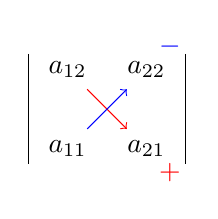
\begin{tikzpicture}
	\draw (0.5,2.2) -- (0.5,0.8);
	\draw (2.5,2.2) -- (2.5,0.8);
      \foreach \x in {1,2}
	\foreach \y in {1,2}
	  {
	      \node at (\x,\y) {$a_{\x\y}$};
	    % \draw (\x,\y) circle (0.2cm);
	    % \fill (\x,\y) circle (0.1cm);
	  }
	  \draw [->, red, shorten <=1em, shorten >=1em] (1,2) -- (2,1);
	  \draw [->, blue, shorten <=1em, shorten >=1em] (1,1) -- (2,2);
	  \foreach \x in {1}{
	      \node[blue] at (\x+1.3,2.3) {$-$};
	      \node[red] at (\x+1.3,0.7) {$+$};
	  }
    \end{tikzpicture}
\end{center}
\end{frame}
%-------------- end slide -------------------------------%}}}
%-------------- start slide -------------------------------%{{{ 7
\begin{frame}[fragile]
\begin{center}
    $3\times 3$
    \bigskip

    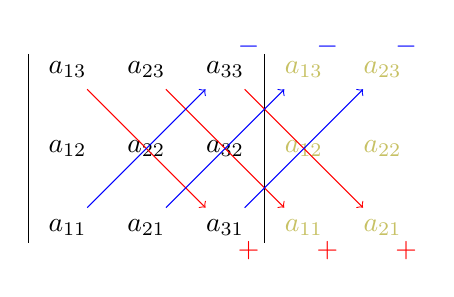
\begin{tikzpicture}
	\draw (0.5,3.2) -- (0.5,0.8);
	\draw (3.5,3.2) -- (3.5,0.8);
	\foreach \x in {1,2,3}
	\foreach \y in {1,2,3}
	  {
	      \node at (\x,\y) {$a_{\x\y}$};
	    % \draw (\x,\y) circle (0.2cm);
	    % \fill (\x,\y) circle (0.1cm);
	  }
	\foreach \x in {1,2}
	\foreach \y in {1,2,3}
	  {
	      \node[yellow!50!gray] at (\x+3,\y) {$a_{\x\y}$};
	    % \draw (\x,\y) circle (0.2cm);
	    % \fill (\x,\y) circle (0.1cm);
	  }
	  \draw [->, red, shorten <=1em, shorten >=1em] (1,3) -- (3,1);
	  \draw [->, red, shorten <=1em, shorten >=1em] (2,3) -- (4,1);
	  \draw [->, red, shorten <=1em, shorten >=1em] (3,3) -- (5,1);

	  \draw [->, blue, shorten <=1em, shorten >=1em] (1,1) -- (3,3);
	  \draw [->, blue, shorten <=1em, shorten >=1em] (2,1) -- (4,3);
	  \draw [->, blue, shorten <=1em, shorten >=1em] (3,1) -- (5,3);
	  \foreach \x in {1,2,3}{
	      \node[blue] at (\x+2.3,3.3) {$-$};
	      \node[red] at (\x+2.3,0.7) {$+$};
	  }
    \end{tikzpicture}
\end{center}
\end{frame}
%-------------- end slide -------------------------------%}}}
%-------------- start slide -------------------------------%{{{ 8
\begin{frame}[fragile]
\begin{center}
    \includegraphics[scale=0.07]{./figures/Determinant_parallelepiped.png}
\end{center}
\vfill
\begin{align*}
    \det \begin{pmatrix} \vec{r}_1 & \vec{r}_2 & \vec{r}_3    \end{pmatrix}
    = \text{signed volume of the parallelepipe}
\end{align*}
\end{frame}
%-------------- end slide -------------------------------%}}}
%-------------- start slide -------------------------------%{{{ 9
\begin{frame}[fragile]
\begin{center}
    $4\times 4$
    \bigskip

    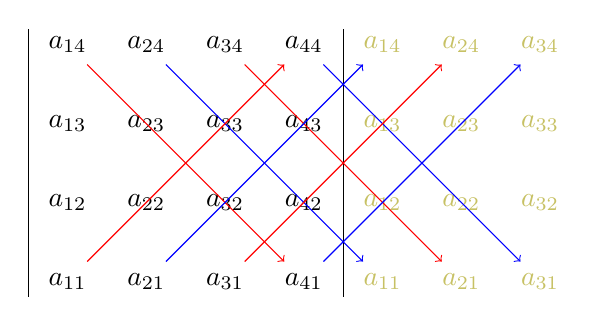
\begin{tikzpicture}
	\draw (0.5,4.2) -- (0.5,0.8);
	\draw (4.5,4.2) -- (4.5,0.8);
      \foreach \x in {1,2,3,4}
	\foreach \y in {1,2,3,4}
	  {
	      \node at (\x,\y) {$a_{\x\y}$};
	    % \draw (\x,\y) circle (0.2cm);
	    % \fill (\x,\y) circle (0.1cm);
	  }
      \foreach \x in {1,2,3}
	\foreach \y in {1,2,3,4}
	  {
	      \node[yellow!50!gray] at (\x+4,\y) {$a_{\x\y}$};
	    % \draw (\x,\y) circle (0.2cm);
	    % \fill (\x,\y) circle (0.1cm);
	  }
	  \draw [->, red, shorten <=1em, shorten >=1em] (1,4) -- (4,1);
	  \draw [->, blue, shorten <=1em, shorten >=1em] (2,4) -- (5,1);
	  \draw [->, red, shorten <=1em, shorten >=1em] (3,4) -- (6,1);
	  \draw [->, blue, shorten <=1em, shorten >=1em] (4,4) -- (7,1);

	  \draw [->, red , shorten <=1em, shorten >=1em] (1,1) -- (4,4);
	  \draw [->, blue, shorten <=1em, shorten >=1em] (2,1) -- (5,4);
	  \draw [->, red , shorten <=1em, shorten >=1em] (3,1) -- (6,4);
	  \draw [->, blue, shorten <=1em, shorten >=1em] (4,1) -- (7,4);
    \end{tikzpicture}
    \end{center}
    \vfill
    \begin{emptytitle}
	\centering
    Only partially right... still missing many terms...
    \end{emptytitle}
\end{frame}
%-------------- end slide -------------------------------%}}}
%-------------- start slide -------------------------------%{{{ 10
\begin{frame}[fragile]
\begin{center}
    $4\times 4$ part I:
    \bigskip

    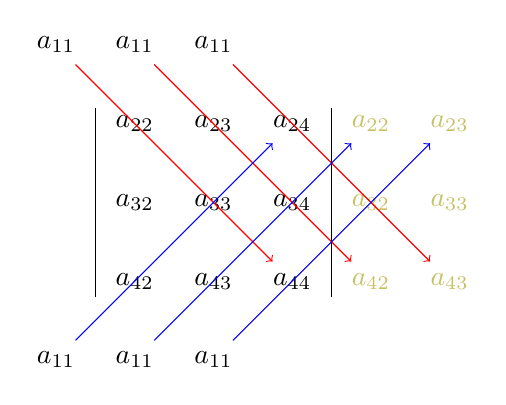
\begin{tikzpicture}
	\draw (0.5,3.2) -- (0.5,0.8);
	\draw (3.5,3.2) -- (3.5,0.8);


	\foreach \x in {0,1,2}
	    \foreach \y in {0,4}
	    {
		  \node at (\x,\y) {$a_{11}$};
	    }
	\foreach \x in {1,2,3}
	    \foreach \y in {1,2,3}
	      {
		  \pgfmathtruncatemacro{\b}{\x+1}%
		  \pgfmathtruncatemacro{\a}{5-\y}%
		  \node at (\x,\y) {$a_{\a\b}$};
		% \draw (\x,\y) circle (0.2cm);
		% \fill (\x,\y) circle (0.1cm);
	      }
	\foreach \x in {1,2}
	    \foreach \y in {1,2,3}
	      {
		  \pgfmathtruncatemacro{\b}{\x+1}%
		  \pgfmathtruncatemacro{\a}{5-\y}%
		  \node[yellow!50!gray] at (\x+3,\y) {$a_{\a\b}$};
		% \draw (\x,\y) circle (0.2cm);
		% \fill (\x,\y) circle (0.1cm);
	      }
	  \draw [->, red, shorten <=1em, shorten >=1em] (0,4) -- (3,1);
	  \draw [->, red, shorten <=1em, shorten >=1em] (1,4) -- (4,1);
	  \draw [->, red, shorten <=1em, shorten >=1em] (2,4) -- (5,1);

	  \draw [->, blue, shorten <=1em, shorten >=1em] (0,0) -- (3,3);
	  \draw [->, blue, shorten <=1em, shorten >=1em] (1,0) -- (4,3);
	  \draw [->, blue, shorten <=1em, shorten >=1em] (2,0) -- (5,3);
    \end{tikzpicture}
\end{center}
\end{frame}
%-------------- end slide -------------------------------%}}}
%-------------- start slide -------------------------------%{{{ 11
\begin{frame}[fragile]
\begin{center}
    $4\times 4$ part II:
    \bigskip

    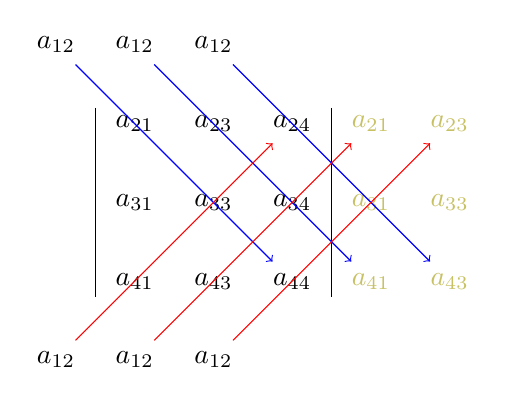
\begin{tikzpicture}
      \draw (0.5,3.2) -- (0.5,0.8);
	\draw (3.5,3.2) -- (3.5,0.8);


	\foreach \x in {0,1,2}
	    \foreach \y in {0,4}
	    {
		  \node at (\x,\y) {$a_{12}$};
	    }
	\foreach \x in {2,3}
	    \foreach \y in {1,2,3}
	      {
		  \pgfmathtruncatemacro{\b}{\x+1}%
		  \pgfmathtruncatemacro{\a}{5-\y}%
		  \node at (\x,\y) {$a_{\a\b}$};
		% \draw (\x,\y) circle (0.2cm);
		% \fill (\x,\y) circle (0.1cm);
	      }
	\foreach \x in {1}
	    \foreach \y in {1,2,3}
	      {
		  \pgfmathtruncatemacro{\b}{\x}%
		  \pgfmathtruncatemacro{\a}{5-\y}%
		  \node at (\x,\y) {$a_{\a\b}$};
		% \draw (\x,\y) circle (0.2cm);
		% \fill (\x,\y) circle (0.1cm);
	      }
	\foreach \x in {1}
	    \foreach \y in {1,2,3}
	      {
		  \pgfmathtruncatemacro{\b}{\x}%
		  \pgfmathtruncatemacro{\a}{5-\y}%
		  \node[yellow!50!gray] at (\x+3,\y) {$a_{\a\b}$};
		% \draw (\x,\y) circle (0.2cm);
		% \fill (\x,\y) circle (0.1cm);
	      }
	\foreach \x in {2}
	    \foreach \y in {1,2,3}
	      {
		  \pgfmathtruncatemacro{\b}{\x+1}%
		  \pgfmathtruncatemacro{\a}{5-\y}%
		  \node[yellow!50!gray] at (\x+3,\y) {$a_{\a\b}$};
		% \draw (\x,\y) circle (0.2cm);
		% \fill (\x,\y) circle (0.1cm);
	      }
	  \draw [->, blue, shorten <=1em, shorten >=1em] (0,4) -- (3,1);
	  \draw [->, blue, shorten <=1em, shorten >=1em] (1,4) -- (4,1);
	  \draw [->, blue, shorten <=1em, shorten >=1em] (2,4) -- (5,1);

	  \draw [->, red, shorten <=1em, shorten >=1em] (0,0) -- (3,3);
	  \draw [->, red, shorten <=1em, shorten >=1em] (1,0) -- (4,3);
	  \draw [->, red, shorten <=1em, shorten >=1em] (2,0) -- (5,3);
    \end{tikzpicture}
\end{center}
\end{frame}
%-------------- end slide -------------------------------%}}}
%-------------- start slide -------------------------------%{{{ 12
\begin{frame}[fragile]
\begin{center}
    $4\times 4$ part III:
    \bigskip

    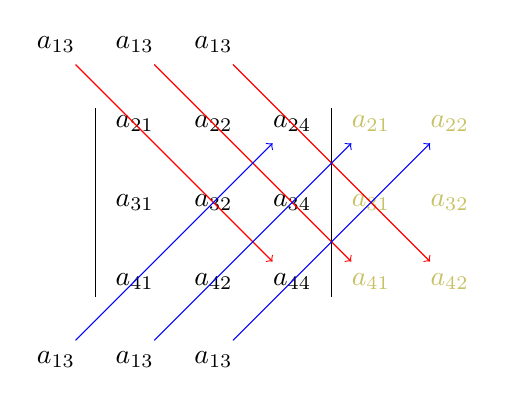
\begin{tikzpicture}
	\draw (0.5,3.2) -- (0.5,0.8);
	\draw (3.5,3.2) -- (3.5,0.8);


	\foreach \x in {0,1,2}
	    \foreach \y in {0,4}
	    {
		  \node at (\x,\y) {$a_{13}$};
	    }
	\foreach \x in {1,2}
	    \foreach \y in {1,2,3}
	      {
		  \pgfmathtruncatemacro{\b}{\x}%
		  \pgfmathtruncatemacro{\a}{5-\y}%
		  \node at (\x,\y) {$a_{\a\b}$};
		% \draw (\x,\y) circle (0.2cm);
		% \fill (\x,\y) circle (0.1cm);
	      }
	\foreach \x in {3}
	    \foreach \y in {1,2,3}
	      {
		  \pgfmathtruncatemacro{\b}{\x+1}%
		  \pgfmathtruncatemacro{\a}{5-\y}%
		  \node at (\x,\y) {$a_{\a\b}$};
		% \draw (\x,\y) circle (0.2cm);
		% \fill (\x,\y) circle (0.1cm);
	      }
	\foreach \x in {1,2}
	    \foreach \y in {1,2,3}
	      {
		  \pgfmathtruncatemacro{\b}{\x}%
		  \pgfmathtruncatemacro{\a}{5-\y}%
		  \node[yellow!50!gray] at (\x+3,\y) {$a_{\a\b}$};
		% \draw (\x,\y) circle (0.2cm);
		% \fill (\x,\y) circle (0.1cm);
	      }
	  \draw [->, red, shorten <=1em, shorten >=1em] (0,4) -- (3,1);
	  \draw [->, red, shorten <=1em, shorten >=1em] (1,4) -- (4,1);
	  \draw [->, red, shorten <=1em, shorten >=1em] (2,4) -- (5,1);

	  \draw [->, blue, shorten <=1em, shorten >=1em] (0,0) -- (3,3);
	  \draw [->, blue, shorten <=1em, shorten >=1em] (1,0) -- (4,3);
	  \draw [->, blue, shorten <=1em, shorten >=1em] (2,0) -- (5,3);
    \end{tikzpicture}
\end{center}
\end{frame}
%-------------- end slide -------------------------------%}}}
%-------------- start slide -------------------------------%{{{ 13
\begin{frame}[fragile]
\begin{center}
    $4\times 4$ part IV:
    \bigskip

    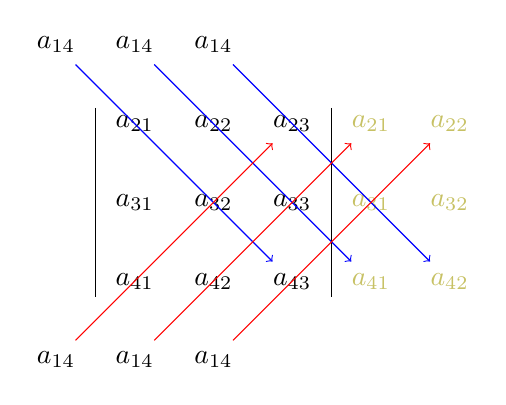
\begin{tikzpicture}
      \draw (0.5,3.2) -- (0.5,0.8);
	\draw (3.5,3.2) -- (3.5,0.8);

	\foreach \x in {0,1,2}
	    \foreach \y in {0,4}
	    {
		  \node at (\x,\y) {$a_{14}$};
	    }
	\foreach \x in {1,2,3}
	    \foreach \y in {1,2,3}
	      {
		  \pgfmathtruncatemacro{\b}{\x}%
		  \pgfmathtruncatemacro{\a}{5-\y}%
		  \node at (\x,\y) {$a_{\a\b}$};
		% \draw (\x,\y) circle (0.2cm);
		% \fill (\x,\y) circle (0.1cm);
	      }
	\foreach \x in {1,2}
	    \foreach \y in {1,2,3}
	      {
		  \pgfmathtruncatemacro{\b}{\x}%
		  \pgfmathtruncatemacro{\a}{5-\y}%
		  \node[yellow!50!gray] at (\x+3,\y) {$a_{\a\b}$};
		% \draw (\x,\y) circle (0.2cm);
		% \fill (\x,\y) circle (0.1cm);
	      }
	  \draw [->, blue, shorten <=1em, shorten >=1em] (0,4) -- (3,1);
	  \draw [->, blue, shorten <=1em, shorten >=1em] (1,4) -- (4,1);
	  \draw [->, blue, shorten <=1em, shorten >=1em] (2,4) -- (5,1);

	  \draw [->, red, shorten <=1em, shorten >=1em] (0,0) -- (3,3);
	  \draw [->, red, shorten <=1em, shorten >=1em] (1,0) -- (4,3);
	  \draw [->, red, shorten <=1em, shorten >=1em] (2,0) -- (5,3);
    \end{tikzpicture}
\end{center}
\end{frame}
%-------------- end slide -------------------------------%}}}
%-------------- start slide -------------------------------%{{{ 14
\begin{frame}[fragile]
\begin{emptytitle}
    $5\times 5$? ... \pause\\[2em]
    The determinant of an $n\times n$ matrix is more effectively defined through recursion...
    % computed using
    % determinants of $(n-1)\times(n-1)$ submatrices.
\end{emptytitle}
\end{frame}
%-------------- end slide -------------------------------%}}}
\section[\textcolor{yellow}{}]{\textcolor{yellow}{The Cofactor Expansion}}
%-------------- start slide -------------------------------%{{{ 15
\frame{
\frametitle{Cofactor and cofactor expansion}
\pause
\begin{definition}
Let $A=\left[ a_{ij}\right]$ be an $n\times n$ matrix.
\begin{itemize}
    \item[--] The \alert{sign} of the $(i,j)$ position is $(-1)^{i+j}$.
	(Thus the sign is $1$ if $(i+j)$ is even, and $-1$ if $(i+j)$ is odd.)
\end{itemize}

\begin{align*}
    \left[ \begin{array}{cccc}
	a_{11} & a_{12} & a_{13} & \cdots \\
	a_{21} & a_{22} & a_{23} & \cdots \\
	a_{31} & a_{32} & a_{33} & \cdots \\
	\vdots & \vdots & \vdots &
    \end{array} \right] \quad \Rightarrow \quad
    \left[ \begin{array}{cccc}
	+      & -      & +      & \cdots \\
	-      & +      & -      & \cdots \\
	+      & -      & +      & \cdots \\
	\vdots & \vdots & \vdots &
    \end{array} \right]
\end{align*}
\end{definition}
}
%-------------- end slide -------------------------------%}}}
%-------------- start slide -------------------------------%{{{ 16
\begin{frame}[fragile]
    \begin{definition}[continued]
    \begin{itemize}
	\item[--] Let $A_{ij}$ denote the $(n-1)\times(n-1)$ matrix obtained from
	$A$ by deleting \alert{row $i$} and \alert{column $j$}. The \alert{$(i,j)$-cofactor} of $A$ is
	\[ c_{ij}(A)=(-1)^{i+j}\det(A_{ij}).\]
    \end{itemize}
    \vfill
    \begin{itemize}
	\item[--] \alert{The determinant of $A$} is defined as
	    \begin{align*}
		\det A = a_{11}c_{11}(A) + a_{12}c_{12}(A) + a_{13}c_{13}(A) + \cdots + a_{1n}c_{1n}(A)
	    \end{align*}
	and is called the \alert{cofactor expansion of $\det A$ along
	row $1$}.
    \end{itemize}
\end{definition}

\end{frame}
%-------------- end slide -------------------------------%}}}
%-------------- start slide -------------------------------%{{{ 17
\frame{
\begin{example}
Let $A=
\left[\begin{array}{rrr}
1 & 2 & 3 \\
4 & 5 & 6 \\
7 & 8 & 9
\end{array}\right]$.
Find $\det A$.
\bigskip

Using cofactor expansion along row 1,
\begin{eqnarray*}
\det A & = & 1c_{11}(A) + 2c_{12}(A) + 3c_{13}(A) \\
& = & 1(-1)^2
\left|\begin{array}{rr}
5 & 6 \\ 8 & 9 \end{array}\right| +
2(-1)^3\left|\begin{array}{rr}
4 & 6 \\ 7 & 9 \end{array}\right| +
3(-1)^4\left|\begin{array}{rr}
4 & 5 \\ 7 & 8 \end{array}\right| \\
& = & (45-48) -2(36-42) +3(32-35) \\
& = & -3 -2(-6)+3(-3) \\
& = & -3 + 12 -9 \\
& = & 0
\end{eqnarray*}
\end{example}
}
%-------------- end slide -------------------------------%}}}
%-------------- start slide -------------------------------%{{{ 18
\frame{
\begin{example}[continued]
$A= \left[\begin{array}{rrr}
1 & 2 & 3 \\
4 & 5 & 6 \\
7 & 8 & 9
\end{array}\right]$
\bigskip

Now try cofactor expansion along column 2.
\uncover<2->{
\begin{eqnarray*}
\det A & = & 2c_{12}(A) + 5c_{22}(A) + 8c_{32}(A) \\
& = & 2(-1)^3
\left|\begin{array}{rr}
4 & 6 \\ 7 & 9 \end{array}\right| +
5(-1)^4\left|\begin{array}{rr}
1 & 3 \\ 7 & 9 \end{array}\right| +
8(-1)^5\left|\begin{array}{rr}
1 & 3 \\ 4 & 6 \end{array}\right| \\
& = & -2(36-42) +5(9-21) -8(6-12) \\
& = & -2(-6) +5(-12) -8(-6) \\
& = & 12 - 60 + 48 \\
& = & 0.
\end{eqnarray*}}

\uncover<3->{
We get the same answer!}
\end{example}
}
%-------------- end slide -------------------------------%}}}
%-------------- start slide -------------------------------%{{{ 19
\frame{
\begin{theorem}[Cofactor Expansion Theorem]
The determinant of an $n\times n$ matrix $A$ can be computed using
the cofactor expansion along \alert{any row or column} of $A$.
\end{theorem}
\vfill
\pause
\begin{example}
Let
$A= \left[\begin{array}{rrrr}
	\textcolor<2->{blue}{0} & \textcolor<2->{blue}{1} & \textcolor<2->{blue}{2} & \textcolor<2->{blue}{1} \\
5 & 0 & 0 & 7 \\
\textcolor<2->{red}{0} & \textcolor<2->{red}{1} & \textcolor<2->{red}{-1} & \textcolor<2->{red}{0} \\
3 & 0 & 0 & 2
\end{array}\right]$.
Cofactor expansion along row 1 yields
\begin{eqnarray*}
    \det A & = & \textcolor{blue}{0}c_{11}(A) + \textcolor{blue}{1}c_{12}(A) + \textcolor{blue}{2}c_{13}(A) + \textcolor{blue}{1}c_{14}(A) \\
	   & = & 1c_{12}(A) + 2c_{13}(A) + c_{14}(A),
\end{eqnarray*}
whereas cofactor expansion along, row 3 yields
\begin{eqnarray*}
    \det A & = & \textcolor{red}{0}c_{31}(A) + \textcolor{red}{1}c_{32}(A) + (\textcolor{red}{-1})c_{33}(A) + \textcolor{red}{0}c_{34}(A) \\
	   & = & 1c_{32}(A) + (-1)c_{33}(A),
\end{eqnarray*}
i.e., in the first case we have to compute three cofactors, but in
the second we only have to compute two.
\end{example}
}
%-------------- end slide -------------------------------%}}}
%-------------- start slide -------------------------------%{{{ 20
\frame{
\begin{example}[continued]
We can save ourselves some work by using cofactor expansion
along row 3 rather than row 1.
\[ A= \left[
	\begin{array}{rrrr}
	    0 & 1         & 2          & 1 \\
	    5 & 0         & 0          & 7 \\
	    0 & \alert{1} & \alert{-1} & 0 \\
	    3 & 0         & 0          & 2
	\end{array}\right]
\]

\begin{eqnarray*}
    \det A & = & \alert{1}c_{32}(A) + (\alert{-1})c_{33}(A)\\
& = & 1 (-1)^5
\left|\begin{array}{rrr}
0 & 2 & 1 \\
5 & 0 & 7 \\
3 & 0 & 2
\end{array}\right| +
(-1)(-1)^6
\left|\begin{array}{rrr}
0 & 1 & 1\\
5 & 0 & 7 \\
3 & 0 & 2
\end{array}\right| \\
& = & (-1)2(-1)^3
\left|\begin{array}{rr}
5 & 7 \\ 3 & 2
\end{array}\right|
+ (-1)1(-1)^3
\left|\begin{array}{rr}
5 & 7 \\ 3 & 2
\end{array}\right| \\
& = & 2(10-21) + 1(10-21)\\
& = & 2(-11) + (-11)\\
& = & -33.
\end{eqnarray*}
\end{example}
}
%-------------- end slide -------------------------------%}}}
%-------------- start slide -------------------------------%{{{ 21
\frame{
\begin{example}[continued]
Try computing
$\det \left[\begin{array}{rrrr}
0 & 1 & 2 & 1 \\
5 & 0 & 0 & 7 \\
0 & 1 & -1 & 0 \\
3 & 0 & 0 & 2
\end{array}\right]$
using cofactor expansion along other rows and columns, for
instance column 2 or row 4.
You will still get $\det A=-33$.
\myQED
\end{example}
}
%-------------- end slide -------------------------------%}}}
%-------------- start slide -------------------------------%{{{ 22
\frame{
\begin{problem}
    Find $\det A$ for
    $A=\left[\begin{array}{rrrr}
	-8 & 1  & 0 & -4 \\
	5  & 7  & 0 & -7 \\
	12 & -3 & 0 & 8  \\
	-3 & 11 & 0 & 2
    \end{array}\right]$.
\end{problem}
\bigskip
\pause
\begin{solution}
    Using cofactor expansion along column 3, $\det A = 0$.\myQED
\end{solution}
\vfill
\pause
\begin{remark}
    If $A$ is an $n\times n$ matrix with a row or column of zeros, then $\det A = 0$.
\end{remark}
}
%-------------- end slide -------------------------------%}}}
\section[\textcolor{yellow}{}]{\textcolor{yellow}{Elementary Row Operations and Determinants}}
%-------------- start slide -------------------------------%{{{ 23
\frame{
\frametitle{Elementary Row Operations and Determinants}
\pause
\begin{example}
    Let $A=\left[\begin{array}{rrr}
	2 & 0 & -3 \\
	0 & 4 & 0 \\
	1 & 0 & -2
    \end{array}\right]$.
    Then
    \uncover<2->{
    \[ \det A=4(-1)^4\left|
    \begin{array}{rr}
    2 & -3 \\ 1 & -2 \end{array}\right|
    = 4(-1)=-4.\]}

    \uncover<3->{
    Let $B_1, B_2$, and $B_3$ be obtained from $A$ by performing a
    type 1, 2 and 3 elementary row operation, respectively, i.e.,
    \bigskip

    \begin{align*}
	\begin{array}{c|c|c}
	    r_2 \leftrightarrow r_3 &
	    -3\times r_3 \to r_3 &
	    2\times r_1 + r_3 \to r_3
	    \\[1em]
	    B_1=
	    \left[\begin{array}{rrr}
		2 & 0 & -3 \\
		1 & 0 & -2\\
		0 & 4 & 0 \\
	    \end{array}\right]
	    &
	    B_2 =
	    \left[\begin{array}{rrr}
		2  & 0 & -3 \\
		0  & 4 & 0 \\
		-3 & 0 & 6
	    \end{array}\right]
	    &
	    B_3=
	    \left[\begin{array}{rrr}
		2 & 0 & -3 \\
		0 & 4 & 0 \\
		5 & 0 & -8
	    \end{array}\right].
        \end{array}
    \end{align*}
    }
\end{example}
}
%-------------- end slide -------------------------------%}}}
%-------------- start slide -------------------------------%{{{ 24
\frame{
\begin{example}[continued]
    \[ \det B_1 = 4(-1)^5\left|
    \begin{array}{rr}
    2 & -3 \\ 1 & -2 \end{array}\right|
    = (-4)(-1)=4 = (-1)\det A.\]

    \uncover<2->{
    \[ \det B_2 = 4(-1)^4\left|
    \begin{array}{rr}
    2 & -3 \\ -3 & 6 \end{array}\right|
    = 4(12-9)=4\times 3=12= -3\det A.\] }

    \uncover<3->{
    \[ \det B_3 = 4(-1)^4\left|
    \begin{array}{rr}
    2 & -3 \\ 5 & -8 \end{array}\right|
    = 4(-16+15)=4(-1)=-4= \det A.\] }
\end{example}
}
%-------------- end slide -------------------------------%}}}
%-------------- start slide -------------------------------%{{{ 25
\frame{
\begin{theorem}[Determinant and Elementary Row Operations]
    Let $A$ be an $n\times n$ matrix.\\[1em]
    \begin{enumerate}
	\item<1-> If $B$ is obtained from $A$ by exchanging two different rows (or columns) of $A$, then $\textcolor{magenta}{\det B=-\det A}$.
	\item<2-> If $B$ is obtained from $A$ by multiplying a row (or column) of $A$ by a scalar $k\in\RR$, then $\textcolor{magenta}{\det B=k\det A}$.
	\item<3-> If $B$ is obtained from $A$ by adding $k$ times one row of $A$ to a different row of $A$ (or adding $k$ times one column of $A$ to a different column of $A$) then $\textcolor{magenta}{\det B=\det A}$.\\[1em]
	\item<4-> If $A$ has a row or column of zeros, then $\textcolor{magenta}{\det A=0}$.
	\item<5-> If two different rows (or columns) of $A$ are identical, then $\textcolor{magenta}{\det A=0}$.
    \end{enumerate}
\end{theorem}
}
%-------------- end slide -------------------------------%}}}
%-------------- start slide -------------------------------%{{{ 26
\frame{
\begin{example}
    \[ \det\left[\begin{array}{rrr}
	1 & 2 & 3 \\
	4 & 5 & 6 \\
	7 & 8 & 9
    \end{array}\right]
    = \left|
    \begin{array}{rrr}
	1 & 2 & 3 \\
	0 & -3 & -6 \\
	0 & -6 & -12
    \end{array}
    \right|
    = \left|
    \begin{array}{rr}
	-3 & -6 \\
	-6 & -12
    \end{array}
    \right|
    = 36-36=0.\]
		\myQED
\end{example}
}
%-------------- end slide -------------------------------%}}}
%-------------- start slide -------------------------------%{{{ 27
\frame{
\begin{example}
\begin{eqnarray*}
    \det\left[\begin{array}{rrrr}
	    3  & 1  & 2 & 4 \\
	    -1 & -3 & 8 & 0 \\
	    1  & -1 & 5 & 5 \\
	    1  & 1  & 2 & -1
    \end{array}\right]
    & = & \left|
    \begin{array}{rrrr}
	0  & -8 & 26 & 4 \\
	-1 & -3 & 8  & 0 \\
	0  & -4 & 13 & 5 \\
	0  & -2 & 10 & -1
    \end{array}
    \right| \\
    & = & (-1)(-1)^3
    \left|
    \begin{array}{rrr}
	-8 & 26 & 4 \\
	-4 & 13 & 5\\
	-2 & 10 & -1
    \end{array}
    \right| \\
    & = &
    \left|
    \begin{array}{rrr}
	0  & -14 & 8 \\
	0  & -7  & 7 \\
	-2 & 10  & -1
    \end{array}
    \right| \\
    & = &  (-2)(-1)^4
    \left|
    \begin{array}{rr}
	-14 & 8 \\
	-7  & 7
    \end{array}
    \right| \\
    & = & -2
    \left|\begin{array}{rr}
	0  & -6 \\
	-7 & 7
    \end{array}
    \right| \\
    & = & (-2)(-42) = 84.
\end{eqnarray*}
		\myQED
\end{example}
}
%-------------- end slide -------------------------------%}}}
%-------------- start slide -------------------------------%{{{ 28
\frame{
\begin{problem}
    If
    $\det
    \left[\begin{array}{ccc}
	a & b & c \\
	p & q & r \\
	x & y & z
    \end{array}\right] = -1$,
    find
    $\det
    \left[\begin{array}{ccc}
	-x   & -y   & -z   \\
	3p+a & 3q+b & 3r+c \\
	2p   & 2q   & 2r   \\
    \end{array}\right]$.
\end{problem}
\pause
\pause
\begin{solution}
    \[ \left|
    \begin{array}{ccc}
	-x   & -y   & -z   \\
	3p+a & 3q+b & 3r+c \\
	2p   & 2q   & 2r   \\
    \end{array}
    \right| =
    (-1)(2)
    \left|
    \begin{array}{ccc}
	x    & y    & z    \\
	3p+a & 3q+b & 3r+c \\
	p    & q    & r    \\
    \end{array}
    \right|
    \]
    \pause
    \[
    = (-2)\left|
    \begin{array}{ccc}
	x & y & z \\
	a & b & c \\
	p & q & r \\
    \end{array}
    \right|
    =(-2)(-1)\left|
    \begin{array}{ccc}
	a & b & c \\
	x & y & z \\
	p & q & r \\
    \end{array}
    \right|
    =2(-1)\left|
    \begin{array}{ccc}
	a & b & c \\
	p & q & r \\
	x & y & z \\
    \end{array}
    \right|
    \]
    \pause
    \hspace*{.19in} $= (-2)(-1)=2$.
    \myQED
\end{solution}
}
%-------------- end slide -------------------------------%}}}
%-------------- start slide -------------------------------%{{{ 29
\frame{
\begin{example}
    \begin{eqnarray*}
	\det \left[
	\begin{array}{rrr}
	    1 & 2 & 3 \\
	    0 & 5 & 6 \\
	    0 & 0 & 9
	\end{array}
	\right]
	& = & 1\det \left[
	\begin{array}{rr}
	    5 & 6 \\
	    0 & 9
	\end{array}
	\right]\\
	& = & (1)(5) \det\left[
	\begin{array}{r}
	9
	\end{array}
	\right]\\
	& = & (1)(5)(9) \\
	& = & 45.
    \end{eqnarray*}
\myQED
\end{example}
}
%-------------- end slide -------------------------------%}}}
\section[\textcolor{yellow}{}]{\textcolor{yellow}{Determinant and Scalar Multiple}}
%-------------- start slide -------------------------------%{{{ 30
\frame{
\frametitle{Determinant and Scalar Multiple}
\pause
\begin{problem}
Suppose $A$ is a $3\times 3$ matrix with $\det A=7$.
What is $\det(-3A)$?
\end{problem}
\pause
\vfill
\begin{solution}
\uncover<2->{
Write
$A=\left[\begin{array}{rrr}
a_{11} & a_{12} & a_{13} \\
a_{21} & a_{22} & a_{23} \\
a_{31} & a_{32} & a_{33}
\end{array}\right]$.
Then
$-3A=\left[\begin{array}{rrr}
-3a_{11} & -3a_{12} & -3a_{13} \\
-3a_{21} & -3a_{22} & -3a_{23} \\
-3a_{31} & -3a_{32} & -3a_{33}
\end{array}\right]$.}

\uncover<3->{
\[ \det(-3A) =
\left|
\begin{array}{rrr}
-3a_{11} & -3a_{12} & -3a_{13} \\
-3a_{21} & -3a_{22} & -3a_{23} \\
-3a_{31} & -3a_{32} & -3a_{33}
\end{array}
\right|
=
(-3) \left|
\begin{array}{rrr}
a_{11} & a_{12} & a_{13} \\
-3a_{21} & -3a_{22} & -3a_{23} \\
-3a_{31} & -3a_{32} & -3a_{33}
\end{array}
\right|
\]}
\uncover<4->{
\[
=(-3)(-3) \left|
\begin{array}{rrr}
a_{11} & a_{12} & a_{13} \\
a_{21} & a_{22} & a_{23} \\
-3a_{31} & -3a_{32} & -3a_{33}
\end{array}
\right|
=(-3)(-3)(-3) \left|
\begin{array}{rrr}
a_{11} & a_{12} & a_{13} \\
a_{21} & a_{22} & a_{23} \\
a_{31} & a_{32} & a_{33}
\end{array}
\right|
\]}

\uncover<5->{
$= (-3)^3 \det A = (-27)\times 7 = -189$.
\myQED
}
\end{solution}
}
%-------------- end slide -------------------------------%}}}
%-------------- start slide -------------------------------%{{{ 31
\frame{
\begin{theorem}[Determinant of Scalar Multiple of Matrices]
If $A$ is an $n\times n$ matrix and $k\in\RR$ is a scalar, then
\[ \det(kA)=k^n\det A.\]
\end{theorem}
}
%-------------- end slide -------------------------------%}}}
%-------------- start slide -------------------------------%{{{ 32
\frame{
\begin{problem}
Let
\[
A=\left[\begin{array}{ccc}
a & b & c \\
p & q & r \\
x & y & z
\end{array}\right]
\quad\text{and}\quad
B=\left[\begin{array}{ccc}
2a+p & 2b+q & 2c+r \\
2p+x & 2q+y & 2r+z \\
2x+a & 2y+b & 2z+c
\end{array}\right]
\]
Show that $\det B= 9\det A$.
\end{problem}
}
%-------------- end slide -------------------------------%}}}
%-------------- start slide -------------------------------%{{{ 33
\frame{
\begin{solution}
$\det B
= \left|\begin{array}{ccc}
2a+p & 2b+q & 2c+r \\
2p+x & 2q+y & 2r+z \\
2x+a & 2y+b & 2z+c
\end{array}\right|
= \left|\begin{array}{ccc}
p-4x & q-4y & r-4z \\
2p+x & 2q+y & 2r+z \\
2x+a & 2y+b & 2z+c
\end{array}\right| $
\medskip

\uncover<2->{
$ = \left|\begin{array}{ccc}
p-4x & q-4y & r-4z \\
9x & 9y & 9z \\
2x+a & 2y+b & 2z+c
\end{array}\right|
= 9\left|\begin{array}{ccc}
p-4x & q-4y & r-4z \\
x & y & z \\
2x+a & 2y+b & 2z+c
\end{array}\right|$}
\medskip

\uncover<3->{
$= 9\left|\begin{array}{ccc}
p & q & r \\
x & y & z \\
2x+a & 2y+b & 2z+c
\end{array}\right|
= 9\left|\begin{array}{ccc}
p & q & r \\
x & y & z \\
a & b & c
\end{array}\right|
= -9\left|\begin{array}{ccc}
a & b & c\\
x & y & z \\
p & q & r
\end{array}\right|$}
\medskip

\uncover<4->{
$ = 9\left|\begin{array}{ccc}
a & b & c\\
p & q & r \\
x & y & z \\
\end{array}\right|
=9\det A.$
\myQED}
\end{solution}
}
%-------------- end slide -------------------------------%}}}
\section[\textcolor{yellow}{}]{\textcolor{yellow}{Determinant of Triangular Matrices}}
%-------------- start slide -------------------------------%{{{ 34
\frame{
\frametitle{ Determinant of Triangular Matrices }
\pause
\begin{theorem}
    If $A=\left[a_{ij} \right]$
    is an $n\times n$ (square, upper or lower) triangular matrix, then
    \[ \det A = a_{11} a_{22} a_{33} \cdots a_{nn},\]
    i.e., $\det A$ is the product of the entries of the main diagonal of $A$.
\end{theorem}
\begin{center}
	
\begin{tikzpicture}[scale=1, transform shape]
	\tikzset{>=latex}
	\filldraw[color=teal] (0,1) -- (1,1) -- (1,0);
	\filldraw[color=teal] (1.5,1) -- (1.5,0) -- (2.5,0);
	\draw[color=yellow,thick] (0,0) rectangle (1,1);
	\draw[color=yellow,thick] (1.5,0) rectangle (2.5,1);
	\node[] (0) at (0.3,0.3) {$0$};
	\node[] (0) at (2.25,0.7) {$0$};
	\end{tikzpicture}
\end{center}
}
%-------------- end slide -------------------------------%}}}
%-------------- start slide -------------------------------%{{{ 35
\begin{frame}
    \begin{center}
      Determinants of  \alert{Upper} Triangular Matrices
    \end{center}
    \vfill
    \begin{align*}
	U = \left[ \begin{array}{cccc}
		u_{11} & u_{12} & \cdots & u_{1n} \\
		0      & u_{22} & \cdots & u_{2n} \\
		\vdots & \vdots & \ddots & \vdots \\
		0      & 0      & \cdots & u_{nn}
	\end{array} \right]
    \end{align*}
    \[\Downarrow\]
    \begin{align*}
	    \mbox{det}(U) = u_{11} u_{22} \cdots u_{nn}
    \end{align*}
\end{frame}
%-------------- end slide -------------------------------%}}}
%-------------- start slide -------------------------------%{{{ 36
\begin{frame}
    \begin{center}
      Determinants of \alert{lower} Triangular Matrices
    \end{center}
    \vfill
    \begin{align*}
	L = \left[ \begin{array}{cccc}
		\ell_{11} & 0         & \cdots & 0 \\
		\ell_{21} & \ell_{22} & \cdots & 0 \\
		\vdots    & \vdots    & \ddots & \vdots \\
		\ell_{n1} & \ell_{n2} & \cdots & \ell_{nn}
	\end{array} \right]
    \end{align*}
    \[\Downarrow\]
    \begin{align*}
	\mbox{det}(L) = \ell_{11} \ell_{22} \cdots \ell_{nn}
    \end{align*}
\end{frame}
%-------------- end slide -------------------------------%}}}
%-------------- start slide -------------------------------%{{{ 37
\begin{frame}
    \begin{center}
      Determinants of \alert{diagonal} Matrices
    \end{center}
    \vfill
    \begin{align*}
	D = \left[ \begin{array}{cccc}
	    d_{11} & 0      & \cdots & 0 \\
	    0      & d_{22} & \cdots & 0 \\
	    \vdots & \vdots & \ddots & \vdots \\
	    0      & 0      & \cdots & d_{nn}
	\end{array} \right]
    \end{align*}
    \[\Downarrow\]
    \begin{align*}
	\mbox{det}(D) = d_{11} d_{22} \cdots d_{nn}
    \end{align*}
\end{frame}
%-------------- end slide -------------------------------%}}}
\section[\textcolor{yellow}{}]{\textcolor{yellow}{Determinant of Block Matrices}}
%-------------- start slide -------------------------------%{{{ 38
\frame{
\frametitle{ Determinant of Block Matrices }
\pause
\begin{theorem}
    Consider the matrices
    \[
    \left[\begin{array}{cc}
    A & X \\ 0 & B \end{array}\right]
    \quad\text{and}\quad
    \left[\begin{array}{cc}
    A & 0 \\ Y & B \end{array}\right]
    \]
    where $A$ and $B$ are square matrices.  Then
    \[ \det \left[\begin{array}{cc}
    A & X \\ 0 & B \end{array}\right]
    =\det A \det B
    \quad\text{and}\quad
    \det \left[\begin{array}{cc}
    A & 0 \\ Y & B \end{array}\right]
    =\det A \det B.
    \]
\end{theorem}
}
%-------------- end slide -------------------------------%}}}
%-------------- start slide -------------------------------%{{{ 39
\frame{
\begin{example} $\det \left[\begin{array}{rrrrr}
    1 & -1 & 2 & 0 & -2 \\
    0 & 1 & 0 & 4 & 1 \\
    1 & 1 & 5 & 0 & 0 \\
    0 & 0 & 0 & 3 & -1 \\
    0 & 0 & 0 & 1 & -1
\end{array}\right] = $
\uncover<2->{
$\det \left[\begin{array}{rrr|rr}
    1 & -1 & 2 & 0 & -2 \\
    0 & 1 & 0 & 4 & 1 \\
    1 & 1 & 5 & 0 & 0 \\ \hline
    0 & 0 & 0 & 3 & -1 \\
    0 & 0 & 0 & 1 & -1
\end{array}\right]$}
\vspace{2em}
\uncover<3->{
\[ \hspace*{1.15in}=\det \left[\begin{array}{rrr}
    1 & -1 & 2 \\
    0 & 1 & 0 \\
    1 & 1 & 5
\end{array}\right]
\det \left[\begin{array}{rr}
    3 & -1 \\
    1 & -1
\end{array}\right]\]}
\vfill
\uncover<4->{
\[ \hspace*{0.75in}=\det \left[\begin{array}{rrr}
    1 & 2 \\
    1 & 5
\end{array}\right]
\det \left[\begin{array}{rr}
    3 & -1 \\
    1 & -1
\end{array}\right]\]}
\vfill
\uncover<5->{
\[ = 3\times (-2) = -6.\]}
\end{example}
}
%-------------- end slide -------------------------------%}}}
\section[\textcolor{yellow}{}]{\textcolor{yellow}{Some More Exercises}}
%-------------- start slide -------------------------------%{{{ 40
\frame{
\frametitle{Some More Exercises}
\pause
\begin{example}[From Exercise]
    Evaluate by inspection.
    \[ \det \left[\begin{array}{ccc}
	a   & b   & c   \\
	a+1 & b+1 & c+1 \\
	a-1 & b-1 & c-1
    \end{array}\right] = \mbox{ ?}\]
    \bigskip
    \pause
    \[ \mbox{row}2 + \mbox{row}3 - 2(\mbox{row}1)
    =\left[\begin{array}{ccc}
    0 & 0 & 0 \end{array}\right]\]
\end{example}
}
%-------------- end slide -------------------------------%}}}
%-------------- start slide -------------------------------%{{{ 41
\frame{
\begin{example}[From Exercise]
\begin{itemize}
    \item[(a)] Find $\det A$ if $A$ is $3\times 3$ and $\det(2A)=6$. \pause
    \item[(b)] Let $A$ be an $n\times n$ matrix.
    Under what conditions is $\det(-A)=\det A$?
\end{itemize}
\end{example}
}
%-------------- end slide -------------------------------%}}}
%-------------- start slide -------------------------------%{{{ 42
\frame{
\begin{example}[From Exercise]
    In each case, prove the statement is true or give a counterexample
    showing that the statement is false.
    \begin{itemize}
    \item[(a)] $\det(A+B)=\det A + \det B$.
    \item<2->[(c)] If $A$ is $2\times 2$, then $\det(A^T)=\det A$.
    \item<3->[(e)] If $A$ is $2\times 2$, then $\det(7A)=49\det A$.
    \item<4->[(g)] $\det(-A)=-\det A$.
    \end{itemize}
\end{example}
}
%-------------- end slide -------------------------------%}}}
\end{document}

